\documentclass[preprint,12pt]{elsarticle}
\usepackage[T1]{fontenc}
\usepackage{lmodern}
\usepackage{amsmath,amssymb,booktabs,array,graphicx,microtype}
\usepackage[hidelinks]{hyperref}
\usepackage{placeins,flafter}
\renewcommand{\floatpagefraction}{0.8}
\journal{Neurocomputing}
\makeatletter
\let\ps@pprintTitle\ps@plain
\makeatother
\newcommand{\cov}{\operatorname{cov}}
\newcommand{\full}{\operatorname{full}}
\begin{document}
\begin{frontmatter}
\title{From Set Prediction to Evidence Selection: An Empirical Study of Surrogate Objectives in Multi-hop RAG}
\ifdefined\WithAuthors
\input{author_frontmatter.tex}
\fi
\begin{abstract}
Evidence-set scorers learn to recognize annotated support, but their predictions ultimately choose contexts for a reader. We examine whether supplied-set discrimination transfers to evidence selection in budgeted multi-hop retrieval-augmented generation. First-, second-, and fourth-order factorization models and a DeepSets control use shared dense candidates, supervision, and a fixed reader. Although the static fourth-order model accurately ranks constructed complete and incomplete sets, it retains complete annotated support on 70.9\% of HotpotQA development questions, below the 82.1\% achieved by a feasible six-paragraph dense reference available to its final decision. A search-aligned continuation trains the deployed scores on a shared pool of final and partial search states; static replay matches its optimizer-update count. On the same 128-question HotpotQA/MuSiQue panel, fourth-order support completeness rises from 55 to 57 questions while answer F1 falls from 0.4181 to 0.3766. In both examined seeds, the largest negative contribution comes from questions retaining complete annotated support, whereas newly complete-support groups contribute positively. Second-order continuation produces small gains over its own static models. Exact ball indexes preserve flat-search choices but increase measured selection time at 128 candidates. These exploratory findings distinguish supplied-set discrimination, selected support, answer quality, and measured execution costs. They support evaluating a surrogate through its induced decisions, without establishing generalization beyond the development materials or a causal effect of support completeness on answers.
\end{abstract}
\begin{keyword}
Retrieval-augmented generation \sep Neural set selection \sep Surrogate objectives \sep Multi-hop question answering \sep Search-aligned learning \sep Empirical evaluation
\end{keyword}
\end{frontmatter}

\section{Introduction}
Evidence selection in multi-hop question answering is a decision over combinations of passages. A set scorer may recognize a supplied combination containing the annotated support, yet rank another combination more highly during search. The selected context then informs a separate decision: the reader's answer. Distinguishing these stages matters when support annotations provide the training signal but answer quality remains the downstream objective.

SetR formulates context construction as set selection~\cite{lee2025setr}; RECOMP learns compression and selective augmentation~\cite{xu2024recomp}; and evidence-chain retrieval models interactions between passages~\cite{zhang2024beam,guo2025interchunk}. These approaches move beyond independent relevance ranking. However, aggregate accuracy on supplied evidence sets does not answer whether a score preserves support when it is optimized over many combinations. Nor does an improvement in the annotation target establish an improvement in reader answers. Support annotations can omit valid alternative evidence and do not directly describe the reader's response to a context.

We study compact neural scorers over frozen dense embeddings under a shared candidate pool, paragraph renderer, reader, and input ceiling. The models differ in interaction structure: a first-order model (H1), second- and fourth-order factorization models (H2 and H4), and a DeepSets control. All learn from complete, incomplete, replaced, and redundant support sets. A search-aligned continuation then supervises the score used for selection on a shared pool of search-generated sets, including final decisions and partial frontiers. Static replay controls the number of additional optimizer updates.

Three research questions organize the comparisons. \textbf{RQ1:} Do scores that distinguish constructed sets retain annotated support when a feasible dense reference is available? \textbf{RQ2:} How does training on actual search states change support selection and answers on the same questions? \textbf{RQ3:} Can exact indexing preserve those choices at lower measured cost? The first two questions address the learned objective and its downstream consequences. The third provides a supporting implementation check, comparing vectorized Flat search with granular-ball and k-means indexes in the conditional scoring space.

The contribution is a linked empirical analysis of these decisions. A feasible dense reference exposes selection errors despite high supplied-pair accuracy. Joint support--answer records show that H4's largest negative F1 contribution occurs among questions retaining complete annotated support, while newly complete-support groups contribute positively. H2 responds differently, with small gains over its own static models under both seeds, and MMR remains competitive. Source-text cases illustrate distinctions hidden by aggregate support counts. All 32 answers in the 16 inspected pairs finish before the output limit, ruling out truncation for those cases only. Exact indexing preserves choices but adds measured runtime at this candidate scale.

These comparisons use exposed development material: the initial static checkpoint selection included the answer panel, and source documents overlap development roles (Section~\ref{sec:data}). The findings characterize the tested support-supervised scorers and reader; they do not rank graph-based RAG systems in general.

\section{Related work}
\subsection{Selecting interacting evidence}
Dense passage retrieval provides a scalable relevance backbone~\cite{karpukhin2020dpr}, while multi-hop retrieval extends the decision beyond a single passage~\cite{xiong2021mdr}. MMR balances relevance and redundancy~\cite{carbonell1998mmr}; coverage-based summarization provides another established formulation of joint selection~\cite{lin2011submodular}. These are important controls because a structured scorer must justify more than selecting several individually relevant passages.

SetR explicitly shifts RAG from ranking to set selection~\cite{lee2025setr}. RECOMP learns to compress or omit retrieved context~\cite{xu2024recomp}. Beam Retrieval learns multi-hop retrieval through a beam~\cite{zhang2024beam}. Guo et al. build an inter-chunk interaction graph and retrieve evidence chains using semantic and structural relations~\cite{guo2025interchunk}. Our study does not reproduce those systems or compare their published scores across incompatible settings. It examines a smaller family of annotation-supervised scorers, keeping their candidates and answer interface fixed while following the induced decisions.

\subsection{Learning scores that will be optimized}
Higher-order factorization machines use efficient ANOVA computations to model interactions~\cite{blondel2016hofm}; DeepSets provides a permutation-invariant set architecture~\cite{zaheer2017deepsets}. We adopt these established building blocks as controlled model families. Neither polynomial interactions nor permutation invariance alone establishes that a learned score preserves the desired ordering among searched sets.

Training on states encountered during search has a long history. Beam-search optimization incorporates beam errors in sequence learning~\cite{wiseman2016bso}, while conservative objective models address exploitation of learned objectives in offline optimization~\cite{trabucco2021com}. Our continuation applies direct preferences to saved final sets and partial frontiers, using known support rather than answer reward. It jointly changes the training examples, ranking loss, and checkpoint criterion. The comparison therefore evaluates that intervention as a whole, not the isolated causal effect of a particular loss term.

RAG-LER uses language-model supervision and confidence weighting to regulate a reranker~\cite{zhai2025ragler}. Its supervisory object differs from our mapped support annotations. This distinction matters when interpreting failure: a support scorer need not represent reader utility, even if it predicts its annotation target well.

\subsection{Retrieval quality, answer quality, and implementation cost}
Tian et al. distinguish topical relevance from downstream utility using IR relevance judgments~\cite{tian2025relevance}. Their evaluation uses an IR collection and semantic answer measures, whereas ours uses mapped multi-hop supports and saved canonical answer EM/F1. The common issue is the transition from retrieved information to generated output; the label semantics and experimental interventions differ.

Center--radius maximum-inner-product bounds provide established tools for pruning search~\cite{ram2012tree}. In this study, a granular ball indexes conditional scoring vectors. It does not represent an independently validated semantic evidence unit. We therefore evaluate preservation of Flat's decisions separately from measured selection time.

\section{Study design and models}
Figure~\ref{fig:design} summarizes the comparison interfaces and the separation of fitting, selection, and evaluation. It depicts the completed study design, not a new RAG architecture; its readouts connect the supplied-set and selected-support comparisons (RQ1), paired answer changes (RQ2), and exact-index checks (RQ3).

\begin{figure}[!htbp]\centering
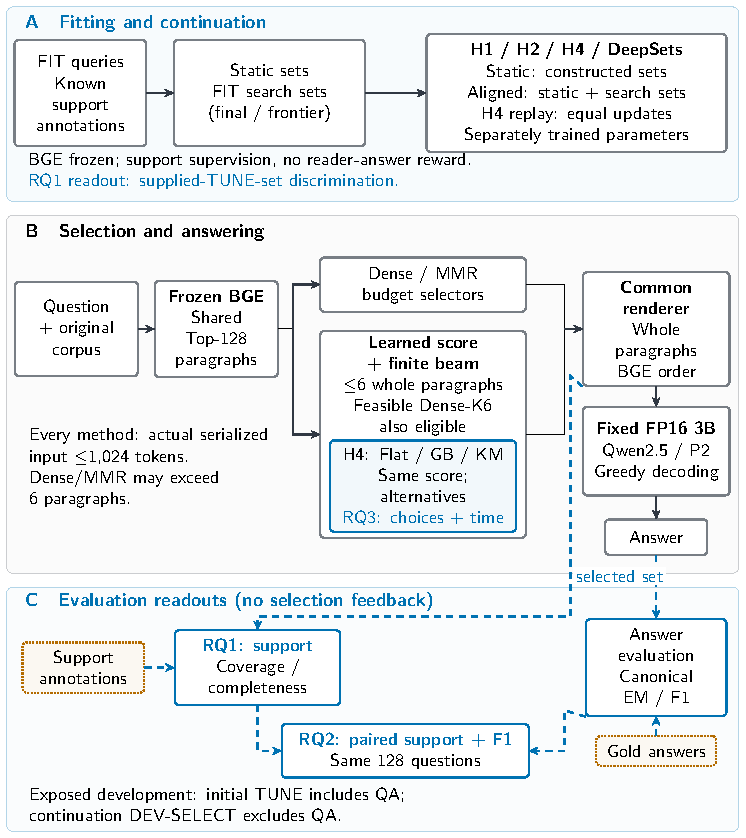
\includegraphics[width=\linewidth]{study_design.pdf}
\caption{Study design and evaluation interfaces. Learned selectors use at most six whole paragraphs; Dense/MMR may exceed six. All share a 1,024-token serialized-input ceiling and BGE display order. Support labels supervise fitting and support evaluation; Gold answers enter answer evaluation only, never selector/reader inputs. Learned factors are not validated semantic relations. H4 Flat, granular-ball (GB), and k-means (KM) implement the same conditional score. This exposed development study includes QA in initial TUNE; only later DEV-SELECT excludes QA. Arrows denote information flow and readouts, not causal effects.}\label{fig:design}
\end{figure}

\subsection{Evidence units and feasible decisions}
For question $q$, a frozen BGE-large-en-v1.5 encoder~\cite{xiao2023bge} retrieves the top 128 paragraphs $V_q$ from a per-dataset development corpus. Every selector sees this same list. Paragraphs are reconstructed from original sentence sources, with the sentence mapping retained for support evaluation. The selected whole paragraphs, including titles, are rendered in their original BGE order.

Let $T(q,S)$ denote the actual tokenizer length of the complete reader input, including question, protocol, and chat framing. Learned selection uses
\begin{equation}\label{eq:feas}
\mathcal F_q=\{S\subseteq V_q:|S|\leq6,\ T(q,S)\leq1024\}.
\end{equation}
An infeasible paragraph is skipped, not truncated to manufacture a feasible set. Tokenization of the assembled input determines feasibility; standalone paragraph lengths are features, not substitutes for this check. The six-paragraph limit and the 1,024-token ceiling are distinct constraints.

Let $G_q$ denote known supporting annotations and $C(S)$ the annotations recovered through the source mapping. The targets are
\begin{equation}\label{eq:targets}
\cov(S)=\frac{|C(S)\cap G_q|}{|G_q|},\qquad
\full(S)=\mathbf 1[G_q\subseteq C(S)].
\end{equation}
These labels describe annotated support. They do not mark every unannotated paragraph as irrelevant, certify factual truth, or guarantee a correct reader answer. Gold annotations are used to construct FIT supervision and evaluate saved outputs; they are not injected into evaluation candidates or supplied to the deployed scorer.

\subsection{Input representation and set scores}
For normalized 1,024-dimensional query and paragraph embeddings $e_q,e_i$, we concatenate $e_q,e_i,e_q\odot e_i,|e_q-e_i|$, cosine relevance, and log paragraph length. Scalar features use FIT normalization statistics. A linear transformation, GELU, and layer normalization produce $h_i\in\mathbb R^{128}$, while a query network produces $h_q$ of the same dimension. Each model has separately trained parameters under this common input design. The features contain no query identifier, target answer, or support-membership flag.

H1, H2, and H4 have full-support and auxiliary coverage heads. For head $t$, the set logit is
\begin{equation}\label{eq:score}
g_{Ht}(S)=b_{qt}(|S|)+\frac{1}{6}\sum_{i\in S}a_{it}
+\sum_{h=2}^{H}\frac{w_{qth}^{\top}E_h(S)}{32\binom{6}{h}},
\end{equation}
where $H\in\{1,2,4\}$ is the maximum interaction order, $t$ denotes the head, $a_{it}$ is a unary score, $b_{qt}$ is a query-conditioned cardinality bias, $w_{qth}\in\mathbb R^{32}$ contains query-conditioned order weights, and
\begin{equation}
E_h(S)=\sum_{i_1<\cdots<i_h,\ i_j\in S}
v_{i_1}\odot\cdots\odot v_{i_h},\qquad v_i\in\mathbb R^{32}.
\end{equation}
Factors use a linear projection, layer normalization, and $\tanh$. The denominators are fixed at the maximum cardinality six. H1 omits the interaction sum, H2 includes pair interactions, and H4 includes orders two through four. Only the full-support logit $g$ selects sets; the coverage head is auxiliary.

The DeepSets control retains the unary and cardinality terms and adds a two-output MLP applied to $[\sum_{i\in S}h_i/6,h_q]$, with hidden width 192. It has 707,922 parameters, compared with 670,640 for H2 and 687,152 for H4. H1 registers 662,384 parameters, but 4,192 in its unused interaction projection do not affect the score. Its effective scored capacity is 658,192 parameters. The models share inputs and supervision, but this is not an exact parameter-count match.

\subsection{Flat search and feasible baselines}
Vectorized Flat search begins with the empty set. At each of six depths, each retained parent proposes its four highest-scoring feasible distinct extensions; the global beam keeps four unique sets. All visited sets, not only surviving parents, remain eligible for the final decision. A feasible Dense-K6 reference is also included. The final choice maximizes $g$, with fewer actual input tokens and then stable paragraph identities breaking ties. Negative increments do not stop expansion. Exact extension ranking does not make this finite beam globally optimal.

Dense-budget traverses the dense list and accepts each paragraph that still fits. MMR-budget uses $0.7e_q^\top e_i-0.3\max_{j\in S}e_i^\top e_j$, skipping infeasible additions. These two baselines may retain more than six short paragraphs. Dense-K6 and MMR-K6 add the learned selectors' cardinality limit. All methods use the same final BGE-order renderer. Consequently, comparisons with budget baselines are shared-ceiling pipeline comparisons; comparisons with K6 references more closely match selection constraints.

\subsection{Exact indexes and their limited guarantee}
The standard ANOVA recurrence computes the interaction terms in Eq.~\ref{eq:score}: it updates $E_h\leftarrow E_h+v_i\odot E_{h-1}$ in descending order, with $E_0=\mathbf1$~\cite{blondel2016hofm}. For a fixed parent $S$, an H4 full-support extension can be expressed as
\begin{equation}
g(S\cup\{i\})=o_q(S)+\theta_q(S)^\top z_i,
\qquad z_i=[a_i/6,v_i].
\end{equation}
Here $o_q(S)$ is constant across candidate additions, and $\theta_q(S)$ collects the conditional unary and interaction coefficients; the head index is omitted for readability. This converts extension ranking into maximum-inner-product search. For an index node $B$ with center $c_B$ and maximum Euclidean radius $r_B$, the standard bound is
\begin{equation}\label{eq:bound}
\max_{i\in B}\theta^\top z_i\leq\theta^\top c_B+\|\theta\|_2r_B.
\end{equation}
It follows directly from Cauchy--Schwarz and $r_B=\max_i\|z_i-c_B\|_2$. An average radius would not suffice. The granular-ball index partitions by farthest pivots; the k-means index uses iterated two-center assignments. Both retain every paragraph, share the bound and token checks, and preserve ties at the pruning boundary.

The bound preserves extension ranking relative to Flat under the same score and feasibility checks. It provides no guarantee for global beam optimality or answer quality. Per-query factor construction, tree building, traversal, and token checks are included in the selection-time comparison in Section~\ref{sec:cost}.

\section{Data, supervision, and interventions}\label{sec:data}
\subsection{Development roles and candidate reachability}
The development material contains 4,000 previously exposed HotpotQA and MuSiQue questions~\cite{yang2018hotpotqa,trivedi2022musique}. The group split yields FIT 3,166, TUNE 738, and historical development 96 (Table~\ref{tab:roles}); FIT contains 3,165 groups. The reconstructed corpora contain 9,791 HotpotQA and 31,130 MuSiQue paragraphs. This is corpus retrieval over the available development material, not full-Wikipedia retrieval. BGE retrieval is exact, without ANN approximation. Its 512-token encoder limit truncates 16 and eight paragraphs, respectively; reader feasibility is checked separately.

\begin{table}[!htbp]
\centering\small
\caption{Development roles and their nesting. MINE is inside FIT; DEV-SELECT and QA are disjoint subsets of TUNE. Initial static checkpoint selection used all TUNE, including QA.}\label{tab:roles}
\begin{tabular}{@{}p{2.5cm}rrp{5.2cm}@{}}\toprule
Role & HotpotQA & MuSiQue & Use \\
\midrule
FIT & 748 & 2,418 & Supervised training \\
TUNE & 196 & 542 & Initial checkpoint loss; selection analysis \\
Historical DEV & 56 & 40 & Earlier exposed development \\
\addlinespace MINE (FIT) & 256 & 256 & Shared search-state pool \\
DEV-SELECT (TUNE) & 64 & 64 & Continuation checkpoint selection \\
QA (TUNE) & 64 & 64 & Saved answer comparison \\
\bottomrule\end{tabular}
\end{table}


The answer panel is drawn from TUNE, which was used to select the initial static checkpoints. Only checkpoint selection for the continuation excludes these questions through a separate DEV-SELECT subset. The answer comparisons therefore remain exploratory development results. The top-level FIT, TUNE, and historical-development question groups are disjoint, but FIT and TUNE share 57 HotpotQA and 4,753 MuSiQue source documents. QA contains 48 HotpotQA bridge and 16 comparison questions, and 32 two-hop and 32 longer-hop MuSiQue questions. Every model and seed reuses these 128 questions.

On TUNE, Top128 contains complete known support for 190/196 HotpotQA and 367/542 MuSiQue questions. Considering the original support paragraphs separately, known support fits the input and cardinality limits for 196/196 and 533/542. Reachability and feasibility are different bottlenecks: a support set may fit but not be retrieved. All questions, including nine budget-infeasible MuSiQue cases, remain in the unconditional results.

\subsection{Static supervised sets}
Static FIT supervision includes complete known-support sets, missing-support sets, same-size replacements, redundant additions, Dense-K6/MMR-K6, and limited random examples. FIT reference construction can append missing support paragraphs and matched distractors to create training sets. This training operation is not used by evaluation or search-state mining, which retain the original Top128.

The base loss combines full-support binary cross-entropy, $0.5$ times sigmoid coverage MSE, $0.25$ times pointwise annotation classification, and $0.25$ times a softplus preference for constructed complete/incomplete pairs of equal cardinality. AdamW uses learning rate $10^{-3}$ and weight decay $10^{-4}$. The initial study retained seeds 1729, 2026, and 426; the continuation comparison uses 1729 and 2026. The third static seed is retained in the numerical supplement but is not relabeled as a continuation run.

Constructed-pair accuracy tests a supplied pair distribution. Actual selection tests an optimized distribution of sets, including combinations never represented by those particular pairs. We therefore report pair accuracy, selected support, reader answers, and cost as distinct endpoints. The same-size training control limits an obvious cardinality shortcut but does not eliminate all length or distribution effects.

\subsection{Shared search-aligned continuation}
MINE contains 512 FIT questions selected by deterministic group hash, balanced across datasets with existing question-type strata retained. Each model searches with its current score. A shared pool merges final sets, high-scoring partial frontiers, Dense-K6/MMR-K6, and at most eight deterministic feasible replacement attempts per trajectory. The deduplicated pool is capped at 64 sets per question, prioritizing model finals and high-scoring frontiers. All four models train on the same pool; no model receives exclusive candidates, stronger supervision, or a different reader.

For the annotation utility $u(S)=[\full(S)+\cov(S)]/2$, a preferred pair has $u(S^+)>u(S^-)$. The added loss directly supervises the deployed logit:
\begin{equation}\label{eq:pref}
\ell(S^+,S^-)=\log\left(1+\exp\left\{0.2[u(S^+)-u(S^-)]-[g(S^+)-g(S^-)]\right\}\right).
\end{equation}
Final-set pairs prefer equal cardinality and token ratios within $[0.8,1.25]$, falling back to equal cardinality. Frontier pairs prefer a shared parent and depth, with same-depth fallback. Missing pair categories are masked. Partial sets with zero full labels can still receive different preferences through coverage, and those preferences affect the deployed score $g$, not merely the auxiliary head.

The continuation loss is $L_{\rm base}+0.5L_{\rm final}+0.5L_{\rm frontier}$. Each query supplies four static and four mined base observations and up to one pair per added category. Losses are normalized within and across queries. Each of at most two rounds permits eight epochs, using AdamW at $3\times10^{-4}$, weight decay $10^{-4}$, query batch eight, and gradient clipping at one. A second round re-mines the selected current models.

The pool does not yield a usable preference for every question. In primary-seed round one, final pairs are unavailable for 171/256 HotpotQA and 115/256 MuSiQue questions; frontier pairs are unavailable for 17 and 42. Every question still supplies base supervision. The supplementary method notes retain the corresponding round-two counts. Thus pool size alone does not measure how many questions receive pairwise supervision.

\subsection{Checkpoint and replay controls}
At epochs two, four, and eight, continuation checkpoints are compared by dataset-equal complete support on DEV-SELECT, then coverage, lower original loss, and earlier checkpoint. Every selected model comes from the first round. QA-answer scores do not enter this decision. H4 static replay uses eight static sets per question and matches the selected aligned H4 checkpoint's optimizer-update count. It does not match total training computation, because the pair terms require additional evaluations. Continuation changes the sampled sets, preference losses, and checkpoint criterion together, so the comparison evaluates the combined intervention rather than isolating a loss term.

\subsection{Reader and paired outcome analysis}
The reader is the original FP16 Qwen2.5-3B-Instruct~\cite{qwen2024release}, with greedy decoding, at most 128 output tokens, and the shared P2 single-answer-field protocol. It uses no relation-front-end adapter. Identical model, input tokens, precision, decoding, and protocol identities permit cached output reuse; cache reuse is not independent generation. Existing canonical EM and token F1, including dataset-specific answer handling, are reused without rescoring or answer cleanup. Format failures remain in the denominator.

We paired completed outputs by question, dataset, model, seed, budget, and protocol. Full-support transitions are $00,01,10,11$, where the first and second digits indicate completeness before and after continuation. F1 changes above $10^{-12}$ or below $-10^{-12}$ define increase or decrease; the tolerance handles floating-point differences. For transition group $A$, its contribution to the observed panel mean is
\begin{equation}\label{eq:decomp}
d_A=\frac{1}{N}\sum_{i\in A}(F1_{i,\rm aligned}-F1_{i,\rm static}),\qquad N=128.
\end{equation}
The four contributions sum to the panel difference. Unlike the within-group mean, $d_A$ uses all 128 questions as its denominator. This is a post hoc descriptive decomposition, not a causal attribution or an inferential test. All four models and both seeds are retained, with per-dataset tables in the supplement.

We grouped saved selection logits into fixed sigmoid bins $[0,.2,\ldots,1]$ and reported counts and annotated completeness, including empty bins. These are search-selected TUNE outputs, not an independent calibration sample. For source-text analysis, we selected 16 distinct H4 questions by a fixed hash within dataset, support-transition, and F1-direction cells: primary-seed gain/harm cells first, then new questions from the second seed, with unchanged cells only if needed. Question and source text were read before saved answers. This outcome-stratified case selection does not estimate population error rates.

\subsection{Reproducibility and research assistance}
The numerical supplement links saved outcomes to paired tables, score bins, and measured costs through deterministic scripts. It contains no new model inference, answer rescoring, or statistical testing. Original model identities, decoding settings, role overlaps, training histories, and cost-accounting scopes are documented separately so that numerical reconstruction is not confused with retraining the system.

OpenAI's ChatGPT and Codex assisted with research planning, implementation and debugging, analysis scripts, and source-text case interpretation. Exact historical backend versions were not retained. Numerical checks compared paired totals and endpoint means with saved records; source-text observations were recorded before consulting the corresponding predictions. This assistant-assisted case review is not independent expert annotation. The data figures are reproducibly rendered from the numerical tables with Matplotlib, using plotting code prepared with Codex assistance; no image-generation model produced experimental data or figure content.

\section{Results}
\subsection{RQ1: Does supplied-set prediction transfer to selection?}
Constructed complete/incomplete pair accuracy is high under the primary seed. H4 achieves 0.9645 on HotpotQA and 0.9464 on MuSiQue; H2 achieves 0.9638/0.9422 and DeepSets 0.9620/0.9482. H1 is lower at 0.9475/0.8978. These values show that the supplied training-style distinction is learnable, but do not establish that H4 ranks the alternatives encountered in search better than its controls.

\begin{table}[!htbp]
\centering\small
\caption{Complete annotated support on all TUNE questions, static H4 versus its feasible Dense-K6 reference, seed 1729. Rates are proportions; lost/gained are question counts relative to Dense-K6. Per-question reference logits were not retained.}\label{tab:reference}
\begin{tabular}{@{}lrrrrr@{}}\toprule
Dataset & $N$ & \shortstack{Dense-K6\\complete rate} & \shortstack{H4\\complete rate} & Lost & Gained \\
\midrule
HotpotQA & 196 & 0.8214 & 0.7092 & 27 & 5 \\
MuSiQue & 542 & 0.2565 & 0.2232 & 42 & 24 \\
\bottomrule\end{tabular}
\end{table}

The feasible-reference comparison makes that distinction concrete (Table~\ref{tab:reference}). Dense-K6 recovers complete annotated support for 82.1\% of HotpotQA TUNE questions, compared with 70.9\% for static H4. Relative to the reference, H4 loses 27 complete cases and gains five. On MuSiQue it loses 42 and gains 24, with completeness 22.3\% versus 25.6\%. Since Dense-K6 is explicitly eligible for final selection, these errors cannot all be attributed to the beam failing to visit that feasible reference.

The reference diagnostic reports no selected H4 score below Dense-K6 (tolerance $10^{-8}$). This local comparison points to the score's ordering of feasible alternatives rather than failure to visit that reference. Only aggregate score differences and support-transition counts are available: the diagnostic did not retain per-question Dense-K6 scores or sets, and paired MMR-K6 scores are also missing. The records therefore support the aggregate comparison, but not a per-question score-gap distribution or a measure of global optimization regret.

\begin{figure}[!htbp]\centering
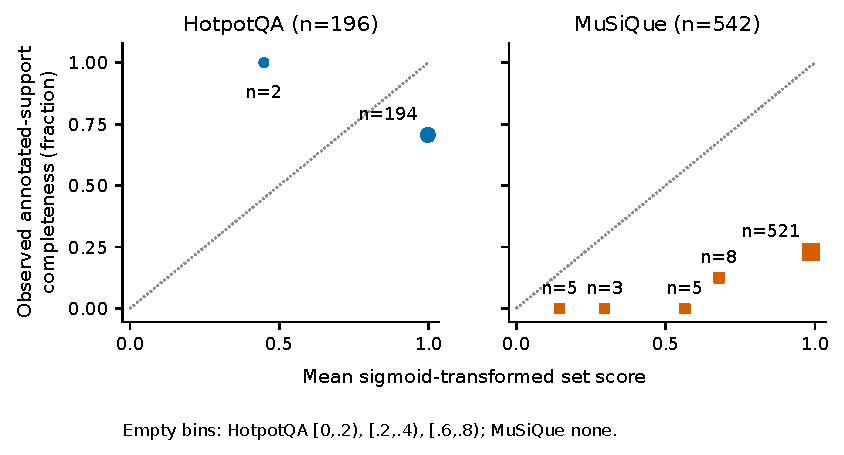
\includegraphics[width=\linewidth]{selected_scores.pdf}
\caption{Sigmoid-transformed scores and observed annotated-support completeness for selected H4 sets, seed 1729. Each point summarizes an occupied fixed bin; labels give its count, and marker area increases with the square root of that count. Empty bins are not interpolated. The diagonal marks equality of the two quantities. These selected TUNE outputs provide a descriptive comparison, not independent calibration.}\label{fig:scores}
\end{figure}

Figure~\ref{fig:scores} shows the discrepancy among saved selected sets directly. In the highest bin, 194 HotpotQA sets have mean sigmoid output 0.9976 but annotated completeness 0.7062. The corresponding 521 MuSiQue sets have mean 0.9867 and completeness 0.2303. The supplement gives the same bins for all four models. Concentration near one is not unique evidence of a high-order failure: the highest DeepSets bins contain 194 and 539 sets, with completeness 0.6959 and 0.2319. Search-selected outputs should therefore not be interpreted as calibrated probabilities from their numeric range alone.

A separate existing matched-length pair diagnostic also limits the higher-order interpretation. H4 pair accuracy is 0.8333/0.7878, compared with 0.9524/0.8525 for DeepSets, on 84/278 pairs from 65/185 queries. This smaller diagnostic changes the supplied-pair distribution and is not a new QA evaluation. Together, the results support a decision-distribution mismatch in the tested scorers; they do not show that adding interactions universally improves evidence choice.

\subsection{RQ2: What changes after search-aligned training?}
\begin{table}[!htbp]
\centering\small
\caption{Answers and contexts on 128 development questions (64 per dataset), seed 1729. Complete support is a question count; F1 and EM are proportions; paragraph and input-token counts are means. Dense/MMR share the 1,024-token ceiling but may exceed six paragraphs. Replay matches optimizer updates.}\label{tab:qa}
\begin{tabular}{@{}lrrrrr@{}}\toprule
Selector & \shortstack{Complete\\support} & F1 & EM & \shortstack{Mean\\paragraphs} & \shortstack{Mean input\\tokens} \\
\midrule
Dense & 64/128 & 0.4055 & 0.3359 & 6.95 & 1009.9 \\
MMR & 61/128 & 0.4303 & 0.3672 & 7.25 & 1007.3 \\
H4 static & 55/128 & 0.4181 & 0.3594 & 5.91 & 916.9 \\
H4-replay & 55/128 & 0.4046 & 0.3359 & 5.91 & 900.9 \\
H1 aligned & 61/128 & 0.4065 & 0.3359 & 4.45 & 696.2 \\
H2 aligned & 56/128 & 0.4057 & 0.3516 & 5.53 & 789.7 \\
DeepSets aligned & 60/128 & 0.4090 & 0.3516 & 4.43 & 693.4 \\
H4 aligned & 57/128 & 0.3766 & 0.2969 & 5.70 & 842.2 \\
\bottomrule\end{tabular}
\end{table}

Table~\ref{tab:qa} retains simple selectors, the static H4 checkpoint, replay, and all aligned models on the same answer panel. MMR has answer F1 0.4303, compared with 0.4181 for static H4 and 0.3766 for aligned H4. H4's complete-support count rises from 55 to 57, but EM falls from 0.3594 to 0.2969. Replay gives F1 0.4046 with 55 complete-support questions. Additional static updates therefore do not reproduce the aligned endpoint, although equal updates are not equal total compute.

The contexts differ in realized size. Dense and MMR average 6.95 and 7.25 paragraphs and about 1,010 and 1,007 input tokens. Static and aligned H4 average 5.91 and 5.70 paragraphs and 917 and 842 tokens. This is a meaningful shared-ceiling comparison but not a context-length-matched answer experiment. Shorter aligned input may reduce reader work, yet the intervention did not isolate length from content. Its F1 change cannot be attributed to shortening alone.

\begin{table}[!htbp]
\centering\small
\caption{Continuation relative to each model's own static checkpoint. Complete-support counts are out of 128; F1 differences use the same full panel. Both seeds reuse the same questions.}\label{tab:paired}
\begin{tabular}{@{}llrrrr@{}}\toprule
Seed & Model & \shortstack{Complete support\\static $\to$ aligned} & \shortstack{Static\\F1} & \shortstack{Aligned\\F1} & $\Delta$F1 \\
\midrule
1729 & H1 & 50 $\to$ 61 & 0.3738 & 0.4065 & +0.0326 \\
1729 & H2 & 47 $\to$ 56 & 0.3998 & 0.4057 & +0.0060 \\
1729 & H4 & 55 $\to$ 57 & 0.4181 & 0.3766 & -0.0415 \\
1729 & DeepSets & 54 $\to$ 60 & 0.4123 & 0.4090 & -0.0033 \\
\addlinespace 2026 & H1 & 49 $\to$ 56 & 0.4277 & 0.4126 & -0.0151 \\
2026 & H2 & 53 $\to$ 54 & 0.4123 & 0.4173 & +0.0051 \\
2026 & H4 & 53 $\to$ 57 & 0.4304 & 0.3831 & -0.0473 \\
2026 & DeepSets & 45 $\to$ 56 & 0.4027 & 0.3521 & -0.0505 \\
\bottomrule\end{tabular}
\end{table}

The response to continuation differs across models (Table~\ref{tab:paired}). Relative to its own static checkpoints, H2 gains 0.0060 and 0.0051 F1 under seeds 1729 and 2026. H1 gains 0.0326 under the first seed but loses 0.0151 under the second. DeepSets and H4 lose F1 under both despite increased complete-support counts. For second-seed H4, full support changes from 53 to 57 and F1 from 0.4304 to 0.3831. The positive H2 differences and negative H4 differences are point estimates on the same development questions, without a significance or equivalence interpretation.

\subsubsection{Joint support--answer transitions}
\begin{figure}[!htbp]\centering
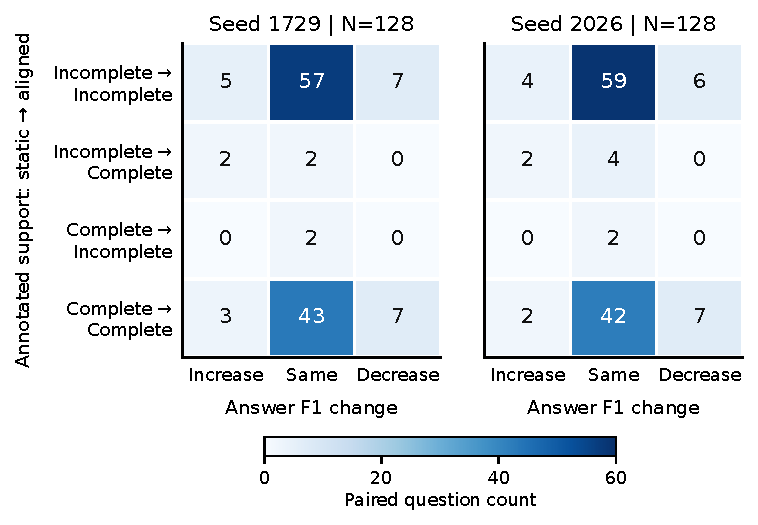
\includegraphics[width=\linewidth]{joint_transitions.pdf}
\caption{Joint changes in annotated-support completeness and answer F1 for H4. Each seed uses the same 128-question panel. Cells show paired counts, including every unchanged case, under a common color scale. Support transitions and F1 directions describe associations between recorded endpoints, not causal effects.}\label{fig:joint}
\end{figure}
Under the primary seed, full support improves for four questions and worsens for two; 122 retain their status. F1 improves for ten, worsens for 14, and remains unchanged for 104. Those margins alone cannot identify which support changes accompany answer changes. Figure~\ref{fig:joint} and Table~\ref{tab:decomp} use their actual intersection.

\begin{table}[!htbp]
\centering\small
\caption{H4 answer-change decomposition by annotated-support transition. Group mean divides the signed sum by group size $n$; panel contribution divides it by all 128 questions. The four contributions sum to the panel difference. Here 0 and 1 mean incomplete and complete annotated support.}\label{tab:decomp}
\begin{tabular}{@{}lcrrrr@{}}\toprule
Seed & \shortstack{Support\\transition} & $n$ & $\sum\Delta$F1 & \shortstack{Group mean\\$\Delta$F1} & \shortstack{Panel\\contribution} \\
\midrule
1729 & 0 $\to$ 0 & 69 & -2.8810 & -0.0418 & -0.0225 \\
1729 & 0 $\to$ 1 & 4 & +1.6667 & +0.4167 & +0.0130 \\
1729 & 1 $\to$ 0 & 2 & +0.0000 & +0.0000 & +0.0000 \\
1729 & 1 $\to$ 1 & 53 & -4.1000 & -0.0774 & -0.0320 \\
\addlinespace 2026 & 0 $\to$ 0 & 69 & -1.1190 & -0.0162 & -0.0087 \\
2026 & 0 $\to$ 1 & 6 & +1.1667 & +0.1944 & +0.0091 \\
2026 & 1 $\to$ 0 & 2 & +0.0000 & +0.0000 & +0.0000 \\
2026 & 1 $\to$ 1 & 51 & -6.1000 & -0.1196 & -0.0477 \\
\bottomrule\end{tabular}
\end{table}

For seed 1729, questions retaining complete annotated support contribute $-0.0320$ to the overall F1 change of $-0.0415$, while the newly complete-support group contributes $+0.0130$. The corresponding contributions for seed 2026 are $-0.0477$ and $+0.0091$, with a total change of $-0.0473$. Every contribution uses all 128 questions as its denominator. The largest negative component therefore lies in the support-preserving group in both runs. The zero contribution of the complete-to-incomplete group and the remaining negative contribution of the incomplete-to-incomplete group are shown in Table~\ref{tab:decomp}. These signed contributions locate the changes; they neither identify a cause nor imply that every question gaining support improved.

Full-support status is binary and intentionally coarse. Within $11$, the selected surrounding paragraphs, wording, ordering under the common renderer, and actual token lengths can still change. Within $00$, partial coverage can change even though completeness remains zero. The decomposition locates changes; it does not identify an internal attention mechanism or establish which context modification caused an answer to change. The numerical supplement retains coverage, EM, paragraph-count, token-count, and context-identity differences for every pair.

\subsubsection{What the source-text cases clarify}
The selected 16 cases were read in full using retained, removed, and added paragraphs before consulting saved predictions. Four illustrate different limits of the aggregate metrics. An added team paragraph supplies the missing conference bridge in C03; support changes $0\to1$ and F1 rises from 0 to 0.6667, while EM remains zero. C12 adds a company-location paragraph tied to the precise role in the question; support changes $0\to1$ and F1 rises from 0 to 1. These are concrete instances in which a recovered bridge accompanies an improved answer.

C10 retains the creator identity and production-date range in both contexts, but the answer changes from the requested production endpoint to a later rights-transfer year in the same source. Full support remains one while F1 drops from one to zero. The text supports a role/date-selection error description, not a claim about why the reader attended to one date. C11 retains a sponsor's full name and acronym; the output switches from the full name to the acronym, with saved canonical F1 changing from one to zero. That lexical change is not equivalent to losing the named entity from the evidence. We retain the original score and do not introduce a favorable alias rule.

All 32 saved answers in the 16 inspected pairs reached the end-of-sequence token before the output limit. Truncation therefore does not explain the changes in these cases. Other cases include unresolved entity links and geographic ambiguity, so a higher answer score alone does not certify a sufficient evidence chain. The supplement reports all 16 observations and their uncertainty. They illustrate plausible reading and lexical-matching errors without estimating their frequency across the full panel.

\subsection{RQ3: Does exact pruning improve actual cost?}\label{sec:cost}
The original index check compared both indexes with Flat on 738 TUNE questions: 1,476 final comparisons and 30,956 extension states showed no mismatch. A fixed refined-leaf diagnostic used 32 questions per dataset and likewise found no mismatch across 128 final comparisons and 2,688 states. These checks assess preservation under the same score and beam, rather than global optimality.

\begin{figure}[!htbp]\centering
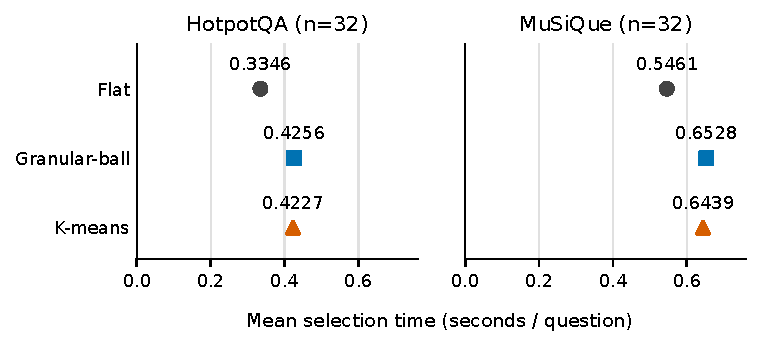
\includegraphics[width=\linewidth]{index_cost.pdf}
\caption{Measured selection time at 128 candidates on a fixed 32-question subset per dataset. Points denote means for Flat and the two exact indexes. Timings include factor construction, per-query indexing, and token-feasibility checks. Some CPU measurements overlapped reader execution, so this is not an isolated hardware benchmark.}\label{fig:cost}
\end{figure}

At 128 candidates, fewer inner-product evaluations did not produce a faster selector (Figure~\ref{fig:cost}). The granular-ball index increased mean selection time from 0.3346 to 0.4256 seconds per HotpotQA question and from 0.5461 to 0.6528 seconds per MuSiQue question. K-means took 0.4227 and 0.6439 seconds, respectively. The granular-ball index reduced mean true extension scores from 2,688 to about 906 and 1,505 but increased tokenizations from 215 to 281 and from 310 to 383. Pruning savings thus coexisted with more feasibility work; the measurements do not isolate either component's causal contribution to total time.

Table~\ref{tab:cost} retains means and medians for the refined 64-question subset. These timings include factor computation, per-query index construction, and tokenizer feasibility checks. Tokenizer time is nested within total selection time and must not be added again. Full process setup and corpus encoding have different accounting scopes. Per-question timing distributions for this subset were not retained; the original 738-question timings are a separate panel in the supplement. Neither panel establishes scaling to a larger corpus or candidate count.

\begin{table}[!htbp]
\centering\small
\caption{Measured selection time in seconds per question, 32 questions per dataset. Means and medians are retained aggregates of the refined-leaf diagnostic; per-question timing distributions are unavailable.}\label{tab:cost}
\begin{tabular}{@{}lrrrr@{}}\toprule
& \multicolumn{2}{c}{HotpotQA} & \multicolumn{2}{c}{MuSiQue} \\ \cmidrule(lr){2-3}\cmidrule(l){4-5}
Selector & Mean & Median & Mean & Median \\
\midrule
Flat & 0.3346 & 0.1694 & 0.5461 & 0.1868 \\
Granular-ball & 0.4256 & 0.2781 & 0.6528 & 0.3005 \\
K-means & 0.4227 & 0.2632 & 0.6439 & 0.2994 \\
\bottomrule\end{tabular}
\end{table}


The supplementary cost ledger reports model-residency GPU wall time, measured CPU time, reader calls, cache reuse, and memory for the broader completed studies. Those totals include development, sensitivity, and repeat work; dividing them by QA's 128 questions would not estimate serving cost. Unrecorded earlier CPU remains unknown.

\section{Discussion and limitations}
\subsection{What the induced decisions reveal}
A feasible dense reference exposes an error that candidate reachability alone cannot explain: the scorer can prefer an alternative with less annotated support even when that reference reaches the final decision. Supplied-pair accuracy therefore leaves an important part of the selection problem unmeasured. The matched-length diagnostic and selected-score bins further indicate that performance depends on the distribution of sets presented to the model. An evaluation should retain an explicit feasible reference alongside constructed examples and searched outputs.

Training on search-generated sets changes the induced choices, but the model-specific responses resist a single higher-order explanation. H2 gains slightly under both seeds, H1 changes direction, and H4 and DeepSets lose answer F1 despite improved completeness counts. The common pool and replay control narrow some alternatives, yet samples, preference losses, and checkpoint criteria change together. These results motivate evaluating the combined training intervention at each decision stage rather than attributing its outcome to one loss or interaction order.

The joint analysis clarifies why aggregate support gains cannot predict the answer change. H4's largest negative contribution comes from questions preserving complete support, while newly complete-support groups contribute positively. A binary annotation target can remain fixed despite changes in paragraph membership, length, and relative position. The cases illustrate an additional distinction between selecting the wrong date role and producing an acronym that loses canonical lexical overlap. Neither requires changing the scoring rule after seeing predictions. Reporting paired support and answer outcomes makes these differences visible.

For implementation choice, the exact indexes preserve decisions but add measured time at this scale. Correctness and fewer inner products are insufficient evidence of practical acceleration. Total measured selector time, with its accounting scope explicit, is the relevant comparison here.

\subsection{Alternative explanations and study boundaries}
The experiments use one frozen encoder, one reader, and one primary 1,024-token interface. Model family, realized context length, and intervention details interact. H4's shorter aligned inputs and different paragraph membership are not isolated factors. MMR and Dense have the same token ceiling but not the same maximum paragraph count; this limits claims of a pure learned-versus-unlearned architecture comparison. The K6 diagnostic establishes a narrower feasible-reference gap in support, without supplying a new K6 answer experiment.

The data are exposed development material. Initial model selection used a TUNE pool containing QA, and source documents overlap FIT and TUNE. Separating later DEV-SELECT does not erase those dependencies. The two seeds reveal sensitivity on the same questions, not two independent confirmation samples. We retain unconditional denominators and do not use a successful-parse, reachable-only, or support-gaining subset as the main answer result. The descriptive analyses add no inferential status to the earlier records.

Support mappings may omit valid alternative evidence. An incomplete annotation set can accompany a correct answer, and complete annotated support can accompany an incorrect or differently phrased answer. Source-text review helps interpret particular cases but is assistant-assisted, outcome-stratified, and limited to 16 questions. It is neither blinded multi-annotator validation nor proof of factual correctness. Per-query Dense-K6 logits and refined-subset timing distributions are missing; the article explicitly distinguishes retained aggregates from newly reconstructible tables.

External graph and hypergraph systems were not run under the same conditions. Their published results cannot establish either an advantage or a failure of the compact scorers evaluated here.

\subsection{Practical implications}
For support-supervised selection, the evidence supports three practical checks: compare searched sets with a feasible simple reference, pair support changes with answers on the same questions, and measure runtime separately from search preservation. MMR and low-order models remain essential controls because neither interaction capacity nor annotation completeness alone explains answer quality. These checks apply to the tested setting without selecting a universally preferable architecture or surrogate.

\section{Conclusion}
This study separates recognizing annotated evidence sets from selecting contexts and using them to answer questions. A feasible dense reference exposes scoring errors that cannot be explained solely by search failing to visit that reference. Training on shared search states changes the induced decisions, but answer effects differ across model families and seeds. H2 shows small gains over its static models, while H4 and DeepSets lose answer F1 despite higher completeness counts. The joint analysis locates H4's largest negative contribution among questions retaining complete annotated support; recovered support contributes positively. This is a description of paired outcomes, not a causal effect of completeness. Exact ball indexes preserve the choices without reducing measured time at 128 candidates. The practical implication is to evaluate learned selectors on the sets they choose, alongside downstream answers, simple controls, and measured costs. These conclusions remain limited to the exposed development material, compact scorers, and shared reader studied here. They do not establish an inherent benefit or failure of higher-order representations.

\ifdefined\WithAuthors
\input{author_credit.tex}
\fi

\section*{Funding}
This research did not receive any specific grant from funding agencies in the public, commercial, or not-for-profit sectors.

\section*{Declaration of generative AI and AI-assisted technologies in the manuscript preparation process}
During manuscript preparation, OpenAI's ChatGPT and Codex were used for literature search and organization, drafting, English revision, and cross-reference checks. The human authors retain responsibility for the article's scientific claims and content. Research uses of these tools are described in the Methods section.

\section*{Declaration of competing interests}
The authors declare that they have no known competing financial interests or personal relationships that could have appeared to influence the work reported in this paper.

\section*{Data availability}
The study uses existing HotpotQA and MuSiQue materials. The accompanying numerical supplement contains de-identified saved scores, paired descriptive tables, source-role information, and a standalone reconstruction script. It reproduces numerical summaries without model inference or access to raw benchmark answers. Source texts, source identities, and trained weights are not bundled. Release of broader derived materials remains subject to source licenses and author approval; no public weight release is claimed.

\bibliographystyle{elsarticle-num}
\bibliography{references,additions,nc_references}
\end{document}
